%% Run LaTeX on this file several times to get Table of Contents,
%% cross-references, and citations.

\documentclass[11pt]{book}
\usepackage{Wiley-AuthoringTemplate}
\usepackage[authoryear]{natbib}%
%for name-date citation comment the below line
%\usepackage[sectionbib,numbers]{natbib}% for numbered citation comment the above line

%%********************************************************************%%
%%       How many levels of section head would you like numbered?     %%
%% 0= no section numbers, 1= section, 2= subsection, 3= subsubsection %%
\setcounter{secnumdepth}{3}
%%********************************************************************%%
%%**********************************************************************%%
%%     How many levels of section head would you like to appear in the  %%
%%				Table of Contents?			%%
%% 0= chapter, 1= section, 2= subsection, 3= subsubsection titles.	%%
\setcounter{tocdepth}{2}
%%**********************************************************************%%

%\includeonly{ch01}
\makeindex

\begin{document}

\frontmatter
%%%%%%%%%%%%%%%%%%%%%%%%%%%%%%%%%%%%%%%%%%%%%%%%%%%%%%%%%%%%%%%%
%% Title Pages
%% Wiley will provide title and copyright page, but you can make
%% your own titlepages if you'd like anyway
%% Setting up title pages, type in the appropriate names here:

%%%%%%%%%%%%%%%%%%%%%%%%%%%%%%%%
\begin{acronyms}
\acro{EM}{Ecological Memory}
\acro{DL}{Deep Learning}
\acro{RNN}{Recurrent Neural Network}
\acro{C}{Carbon}
\acro{LSTM}{Long-Short Term Memory}
\end{acronyms}

\setcounter{page}{1}

\mainmatter

\chapter{Understanding Ecological Memory With Recurrent Neural Networks}

    Ecological memory (EM) can be defined as the ability of the past environmental conditions to influence the current structure and functioning of an ecosystem \cite{CR1,CR2}. In other words, understanding EM provides insights on how past conditions influence ecosystem functioning after those conditions no longer persist. EM can be paritioned into external memory (e.g. soil moisture and air temperature) and internal memory (e.g. species composition and vegetation development stage), which may be encoded across a range of both spatial and temporal scales, from small patch-scale to broad landscapes and spanning from days to decades. In this chapter, we cover topics related to EM for Earth System Science by providing a proof of concept demonstrating the usefulness of dynamic Deep Learning (DL) methods, such as Recurrent Neural Networks (RNNs), for better understanding EM. 

    In the next section (section 1.1), a brief overview of the relevance of understanding EM in Earth system science is provided with an emphasis on ecoystem functioning and hydrological dynamics. A brief description on the use of RNNs model for understanding EM is also provided. 

\section{Ecological memory effects: concepts and relevance} 

	As previously mentioned, ecosystem functioning is not only driven by contemporary environmental conditions, but also by antecedent conditions that are not directly enconded on proxies describing present vegetation's state (e.g. vegetation greenness) and climatic conditions (e.g. air temperature, precipitation) \citep{CR3}. As suggested by \citet{CR4}, the ecosystems are not only responding to direct and indirect concurrent mechanisms but also to direct and indirect lag effects of vegetation and climate fluctuations. For instance, the direct effects can be related to a decrease in productivity during a drought event, while indirect concurrent effects can result in biomass loss from fire facilitated by an ongoing drought (Fig. \ref{fig:14.1}). A drought event can further negatively or positively impact the productivity of an ecosystem from months to years following this event, that is direct lag effects. A common example of indirect lag effects is the occurrence of insect outbreaks that are facilitated by past disturbance events (e.g. drought causes tree mortality and deadwood accumulation, which further contribute to insect outbreaks). The subsequent observed behavior of an ecosystem post-disturbance can depend on a series of complex mechanisms related to the temporal context pre- and post-disturbance, such as the magnitude of the disturbance, the recovery capacity of an ecosystem, its state pre-disturbance, and the environmental conditions (Fig. \ref{fig:14.1}).

    Empirically, the vegetation and climate's EM on ecosystem functioning has been observed. For instance, spring temperature seems to have variable EM on subsequent summer and autumn ecosystem productivity \citep{CR5}, while \citet{CR6} found a dependency of the current ecosystem functioning to previous year water limitation. Additionally, antecedent soil moisture has been shown to control ecosystem responses to changes in concurrent soil moisture \citep{CR15,CR16}. This implies that it is relevant to incorporate these short- to long-term processes to diagnose the functioning of terrestrial ecosystems, albeit it is currently challenging.  

    \begin{figure}[!ht]
    \centering
    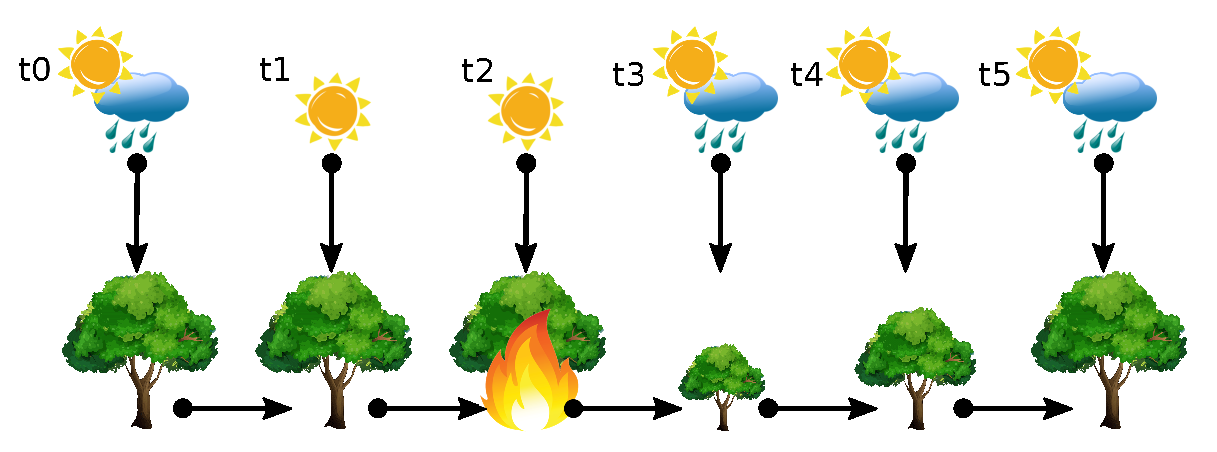
\includegraphics[scale=.6]{figs/Fig1.eps}
    \caption{\textbf{Schematic diagram illustrating the temporal forest dynamics during and post drought conditions.}}
    \label{fig:14.1}
    \end{figure} 

    The concurrent effects of vegetation and climate on biosphere-atmosphere responses have been well observed and described across ecosystems. For instance, extreme temperatures (e.g. heat waves, frost) or unusual warming events have variable effects on the response patterns of photosynthesis and ecosystem respiration to climate extremes. These events can damage a plant, ultimately changing the growth and development of the plant \citep{CR7,CR8,CR9}, or can even perturb the timing of seasonal plant development (e.g. earlier onset of the growing season due to warm late winters) \citep{CR10}. Although evidence points at the need to understand the sensitivity of global ecosystems to recent-past environmental conditions, the scientific community has had less success in understanding EM compared to concurrent effects mainly due to the complex non-linear responses of ecosystems to recent-past climate and vegetation variability. Consequently, the direct and indirect EM of, for instance, climate extremes and past disturbances in the trajectories of terrestrial ecosystems' C dynamics are still poorly understood \citep{CR11}.

\section{On the use of RNNs for understanding ecological memory effects}
    
    A series of data-driven statistical models have intended to account for EM. A common practice to incorporate these dynamic effects is to derive hand-designed variables in machine learning methods, such as lag variables \citep{CR12,CR13}. However, this practice is, most of the time, being applied for only one variable, therefore overlooks the interactive EM between variables \citep{CR14} limiting our capacity to characterize the non-linear feedback between recent-pasrt conditions and ecosystem responses.  Alternatively, the use of non-linear mixed effects model using Bayesian frameworks \citep{CR17,CR2} have shown promising avenues for understanding environmental and biological EM. 

    The recent development of dynamic DL methods, such as RNNs models \citep{CR19,CR20}, enables the extraction of vegetation and climate temporal features that are key to understand ecosystem responses to past environmental conditions (Fig. \ref{fig:14.1}). Such a dynamic approach had success in sequence learning (e.g. speech recognition) and land cover classification \citep{CR21}. The increasing availability of long-term remote sensing products, and climate model simulation outputs opens new avenues to represent long-term climate and vegetation dynamics. Coupled with long‐term ecological observations (e.g. FLUXNET network), the integration of long-term climate and vegetation data into temporally dynamic statistical methods (e.g. RNNs models) may enable the consideration of climate and vegetation's ecological memory effects when modelling and understanding ecoystem functioning. Although the application of RNNs models in Earth System Science is still in its early stage \citep{CR22,CR23,CR24}, such method have shown interesting opportunities to dynamically incorporate the effects of ecosystem history (i.e. recent and past vegetation and climate's dynamics) on ecosystem functioning.     

\begin{figure}[!ht]
    \centering
    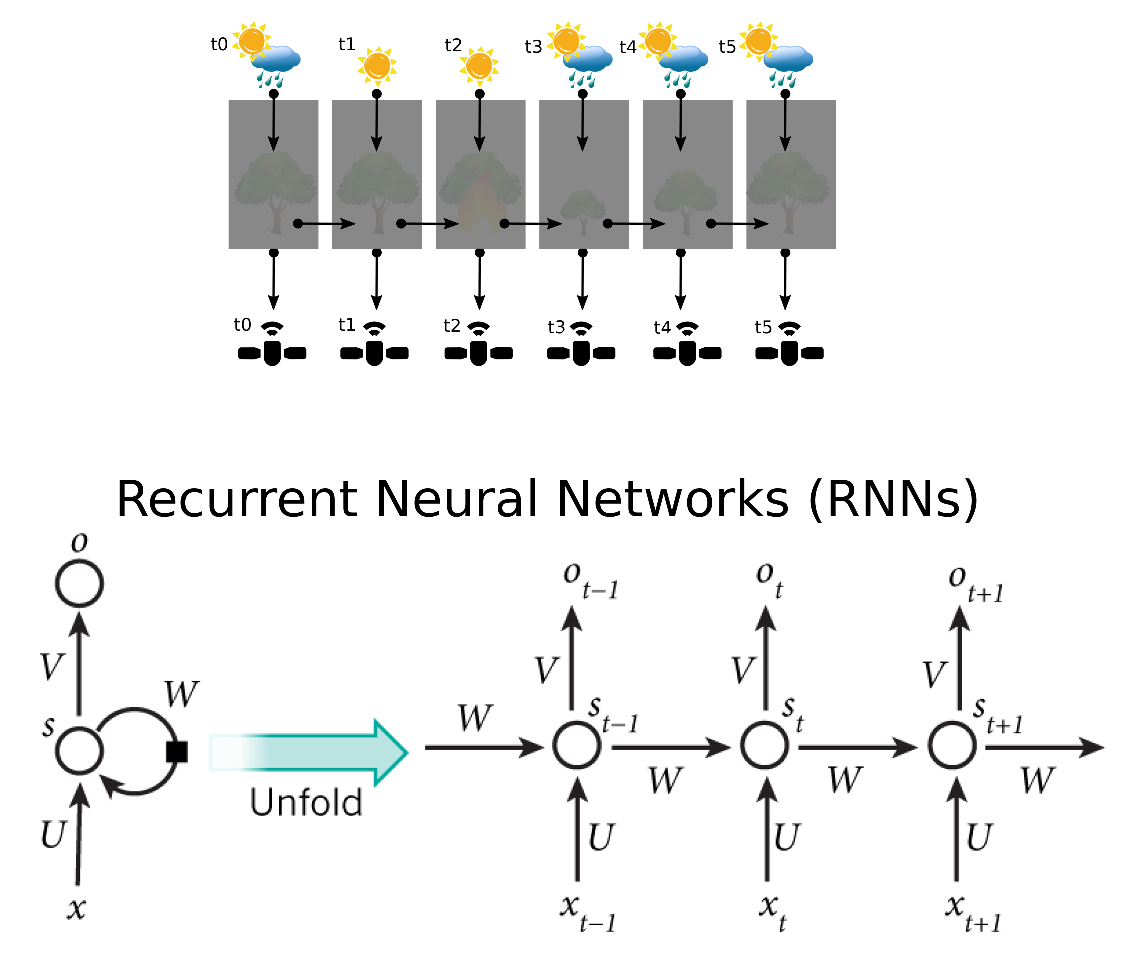
\includegraphics[scale=.6]{figs/Fig2.eps}
    \caption{\textbf{Schematic diagram illustrating the analogy between RNNs architecture and the concept of EM.}}
    \label{fig:14.2}
\end{figure}

\section{Proof of concept}

    In this section, we present the aforementioned proof of concept in which a series of experiments are desribed. These experiments aim at showing (i) the capacity of RNNs to emulate physical model outputs, (ii) the sensitivity of RNNs to noise in both the inputs and model outputs, an (iii) the capacity of RNNs to generalize for unknown conditions.    

\subsection{Material and methods}

    \begin{table}[!ht]
    \begin{tabular}{l|l|l}
    & Hydrological experiment & Vegetaion experiment \\ \hline
    Spatial & PFT &  \\
    Spatial and seasonal & Cloud cover, LAI &  \\
    Spatial, seasonal and interannual & precipation, air temperature, etc & 
    \end{tabular}
    \end{table}

\subsection{Experimental design}

    \begin{figure}[!ht]
    \centering
    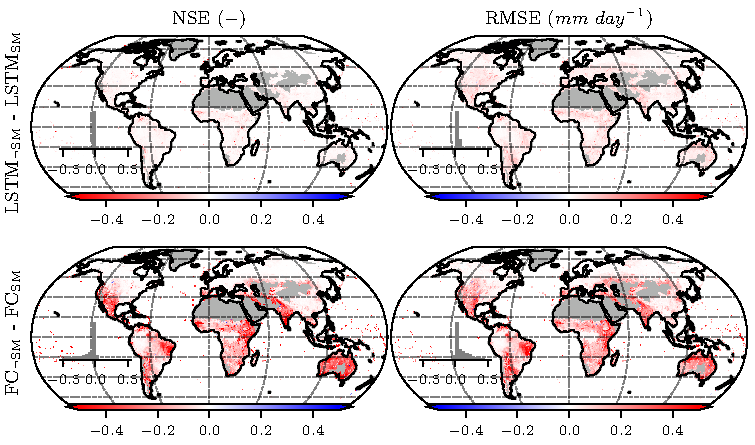
\includegraphics[scale=.6]{figs/Fig3.eps}
    \caption{\textbf{Schematic diagram illustrating the temporal cross-validation.}}
    \label{fig:14.3}
    \end{figure}

\subsection{Results and discussion}

    \begin{figure}[!ht]
    \centering
    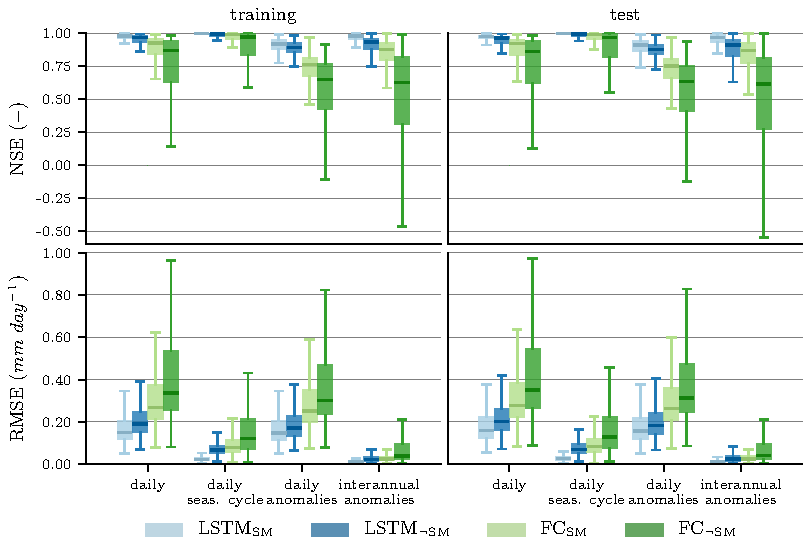
\includegraphics[scale=.6]{figs/Fig4.eps}
    \caption{\textbf{Spatial patterns of model outputs + scatterplots}}
    \label{fig:14.4}
    \end{figure}

    \begin{figure}[!ht]
    \centering
    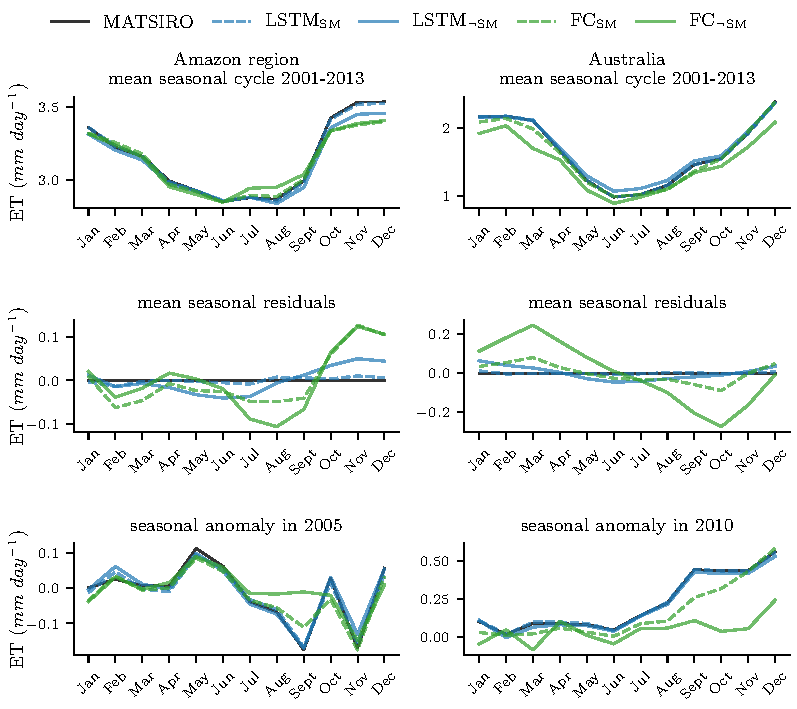
\includegraphics[scale=.6]{figs/Fig5.eps}
    \caption{\textbf{Zoom into specific drought event in 2000s}}
    \label{fig:14.5}
    \end{figure}

    \begin{figure}[!ht]
    \centering
    \includegraphics[scale=.6]{figs/Fig6.eps}
    \caption{\textbf{Drought simulation}}
    \label{fig:14.6}
    \end{figure}

    \begin{table}[!ht]
    \begin{tabular}{l|ll|ll}
    & \multicolumn{2}{c|}{\textbf{Hydrological experiment}} & \multicolumn{2}{c}{\textbf{Vegetaion experiment}} \\
    & \multicolumn{1}{c}{MEF} & \multicolumn{1}{c|}{RMSE} & \multicolumn{1}{c}{MEF} & \multicolumn{1}{c}{RMSE} \\ \hline
    No noise &  &  &  &  \\
    Noise A &  &  &  &  \\
    Noise B &  &  &  & 
    \end{tabular}
    \end{table}

\section{Conclusions}

\backmatter

\bibliography{wiley}%

 
\latexprintindex

\end{document}
